%%%%%%%%%%%%%%%%%%%%%%%%%%%%%%%%%%%%%%%%%%%%%%%%%%%%%%%%%%%%%%%%%%%%%%%%%%%%%%%
%  Formalization and physics: a new frontier for AI
%  Joseph Tooby-Smith -- University of Bath, September 2026
%
%  Compile with: pdflatex BathSeptember26.tex   (run twice)
%%%%%%%%%%%%%%%%%%%%%%%%%%%%%%%%%%%%%%%%%%%%%%%%%%%%%%%%%%%%%%%%%%%%%%%%%%%%%%%
\documentclass[aspectratio=169,10pt]{beamer}

\usepackage[T1]{fontenc}
\usepackage[utf8]{inputenc}
\usepackage[sfdefault]{FiraSans}
\usefonttheme[onlymath]{serif}
\usepackage{amsmath,amssymb}
\usepackage{tikz}
\usepackage{graphicx}
\usepackage{listings}
\usepackage{fontawesome5}
\usepackage[most]{tcolorbox}
\usetikzlibrary{calc,positioning,fadings,arrows.meta,shadows}
% radial falloff, so the background glows read as light rather than as discs
\tikzfading[name=plglow, inner color=transparent!0, outer color=transparent!100]

\graphicspath{{../Images/}{Images/}}

% Clickable links, sane PDF metadata, no ugly boxes.
\hypersetup{
  pdftitle={Formalization and physics: a new frontier for AI},
  pdfauthor={Joseph Tooby-Smith},
  pdfsubject={Formalization, Lean, and physics},
  pdfkeywords={Lean, Physlib, formalization, Standard Model, AI},
  colorlinks=false, pdfborder={0 0 0},
}

%%%%%%%%%%%%%%%%%%%%%%%%%%%%%%%%%%%%%%%%%%%%%%%%%%%%%%%%%%%%%%%%%%%%%%%%%%%%%%%
%  PALETTE  (PhysLib house style)
%%%%%%%%%%%%%%%%%%%%%%%%%%%%%%%%%%%%%%%%%%%%%%%%%%%%%%%%%%%%%%%%%%%%%%%%%%%%%%%
\definecolor{plnavy}  {HTML}{24476B}
\definecolor{plblue}  {HTML}{3D6B99}
\definecolor{plsky}   {HTML}{6FA3CE}
\definecolor{plorange}{HTML}{EF6B3B}
\definecolor{plrust}  {HTML}{D95729}
\definecolor{plgreen} {HTML}{3FA56A}
\definecolor{plpaper} {HTML}{F7FAFD}
\definecolor{plink}   {HTML}{243447}
\definecolor{plmuted} {HTML}{5C7187}
\definecolor{plrule}  {HTML}{C7DCED}
% plorange is a fill/icon colour: too light to set small text on white.
% plember is its text-weight sibling, used wherever orange has to be read.
\definecolor{plember} {HTML}{B0421B}

%%%%%%%%%%%%%%%%%%%%%%%%%%%%%%%%%%%%%%%%%%%%%%%%%%%%%%%%%%%%%%%%%%%%%%%%%%%%%%%
%  BACKGROUNDS
%%%%%%%%%%%%%%%%%%%%%%%%%%%%%%%%%%%%%%%%%%%%%%%%%%%%%%%%%%%%%%%%%%%%%%%%%%%%%%%
% A faint dot lattice -- reads as "structure" without competing with content.
\newcommand{\pldotgrid}[2]{%
  \foreach \x in {0,0.60,...,16.2}{%
    \foreach \y in {0,0.60,...,9.4}{%
      \fill[#1,opacity=#2] ([shift={(\x cm,\y cm)}]current page.south west) circle (0.42pt);}}%
}

% One background for the whole deck: navy gradient, dot lattice, soft glows,
% faint orbital arcs, and a progress bar along the foot.
% The glows use "fade out" so they read as light, not as hard-edged discs.
\newcommand{\plBackground}{%
  \begin{tikzpicture}[remember picture,overlay]
    \shade[top color=plnavy!95, bottom color=plnavy!74]
      (current page.south west) rectangle (current page.north east);
    \begin{scope}
      \clip (current page.south west) rectangle (current page.north east);
      \pldotgrid{white}{0.85}
      \fill[plsky,   opacity=0.30, path fading=plglow]
        ([shift={(-2.0cm,-1.0cm)}]current page.north east) circle (7.6cm);
      \fill[plorange,opacity=0.24, path fading=plglow]
        ([shift={( 0.4cm,-0.2cm)}]current page.south west) circle (6.2cm);
      \foreach \r in {3.2,4.4,5.6,6.8}{%
        \draw[white,opacity=0.07,line width=0.7pt]
          ([shift={(-1.2cm,-0.6cm)}]current page.north east) circle (\r cm);}
    \end{scope}
    % progress bar: how far through the deck we are
    \pgfmathsetmacro{\plfrac}{\insertframenumber/\inserttotalframenumber}%
    \fill[plsky!30!plnavy] (current page.south west)
      rectangle ([yshift=0.16cm]current page.south east);
    \fill[plorange] (current page.south west)
      rectangle ([xshift=\plfrac\paperwidth,yshift=0.16cm]current page.south west);
  \end{tikzpicture}%
}

\setbeamertemplate{background}{\plBackground}

%%%%%%%%%%%%%%%%%%%%%%%%%%%%%%%%%%%%%%%%%%%%%%%%%%%%%%%%%%%%%%%%%%%%%%%%%%%%%%%
%  BEAMER FURNITURE
%%%%%%%%%%%%%%%%%%%%%%%%%%%%%%%%%%%%%%%%%%%%%%%%%%%%%%%%%%%%%%%%%%%%%%%%%%%%%%%
\setbeamertemplate{navigation symbols}{}
\setbeamersize{text margin left=0.62cm,text margin right=0.62cm}
\setbeamercolor{normal text}{fg=plink}
\setbeamercolor{frametitle}{fg=white}
\setbeamercolor{itemize item}{fg=plblue}
\setbeamerfont{frametitle}{size=\LARGE,series=\bfseries}
\setbeamertemplate{itemize item}{\raisebox{0.15ex}{\tiny$\blacksquare$}}
\setlength{\parskip}{2pt}
\setlength{\leftmargini}{1.2em}
% displayed maths inside cards should hug its surroundings, not float in space
\setlength{\abovedisplayskip}{4pt}
\setlength{\belowdisplayskip}{2pt}
\setlength{\abovedisplayshortskip}{4pt}
\setlength{\belowdisplayshortskip}{2pt}

\setbeamertemplate{frametitle}{%
  \vspace*{0.34cm}%
  \begin{minipage}{\dimexpr\paperwidth-1.4cm\relax}
    \raggedright
    {\usebeamerfont{frametitle}\usebeamercolor[fg]{frametitle}\insertframetitle\par}
    \vspace{4pt}
    {\color{plorange}\rule{1.4cm}{2.4pt}}{\color{plsky!40!plnavy}\rule{\dimexpr\linewidth-1.4cm\relax}{2.4pt}}
  \end{minipage}\par\vspace{0.16cm}%
}

\setbeamertemplate{footline}{%
  \hbox{%
    \begin{beamercolorbox}[wd=\paperwidth,ht=2.0ex,dp=3.6ex,leftskip=0.62cm,rightskip=0.62cm]{}%
      {\scriptsize\color{plsky!25!white}Joseph Tooby-Smith\;\textbullet\;University of Bath}%
      \hfill
      {\scriptsize\color{plsky!25!white}\textbf{\insertframenumber}\,/\,\inserttotalframenumber}%
    \end{beamercolorbox}}%
}

%%%%%%%%%%%%%%%%%%%%%%%%%%%%%%%%%%%%%%%%%%%%%%%%%%%%%%%%%%%%%%%%%%%%%%%%%%%%%%%
%  CARDS
%%%%%%%%%%%%%%%%%%%%%%%%%%%%%%%%%%%%%%%%%%%%%%%%%%%%%%%%%%%%%%%%%%%%%%%%%%%%%%%
\tcbset{
  plbase/.style={
    enhanced, arc=6pt, outer arc=6pt, boxrule=0pt, leftrule=4pt,
    colback=white, left=10pt, right=10pt, top=8pt, bottom=8pt,
    halign=flush left,
    drop fuzzy shadow={black!55}, before skip=4pt, after skip=4pt,
  }
}
% Each argument: [extra tcolorbox options] {accent colour} {heading}
\newtcolorbox{plcard}[3][]{plbase, colframe=#2, #1,
  before upper={{\bfseries\color{#2}#3}\par\vspace{5pt}}}
% fixed-height variant, so a row of cards lines up
\newtcolorbox{plcardh}[4][]{plbase, colframe=#2, height=#4, #1,
  before upper={{\bfseries\color{#2}#3}\par\vspace{5pt}}}
\newtcolorbox{plplain}[2][]{plbase, colframe=#2, #1}

% big tinted panel
\newtcolorbox{plpanel}[2]{enhanced, arc=10pt, outer arc=10pt, boxrule=1.2pt,
  colframe=#1!45, colback=#1!7, left=10pt, right=10pt, top=10pt, bottom=10pt,
  before skip=3pt, after skip=3pt, halign=center, valign=center, height=#2,
  drop fuzzy shadow={black!55}}

% one line of a diff, GitHub-style
\newtcolorbox{pldiff}[1]{enhanced, arc=2pt, boxrule=0pt, colback=#1!11,
  colframe=#1!11, left=6pt, right=6pt, top=3pt, bottom=3pt,
  before skip=2pt, after skip=2pt}

% One type scale for the whole deck, so the same kind of text is the same
% size on every slide:
%   \plbody  -- body text inside a card
%   \plmeta  -- captions, attributions, stat rows, small print
%   \pllabel -- the small bold label that sits above a block
\newcommand{\plbody}{\small}
\newcommand{\plmeta}{\footnotesize}
\newcommand{\pllabel}{\footnotesize\bfseries}

\newcommand{\plchip}[2]{%
  \tikz[baseline=(t.base)]{\node[fill=#1!85!black,text=white,rounded corners=5pt,
    inner xsep=5pt,inner ysep=1.8pt,font=\bfseries\scriptsize] (t) {#2};}}

% a bigger badge, for when chips are the main content of a slide (e.g. a
% directory/topic grid) rather than a small label on a card
\newcommand{\plchipbig}[2]{%
  \tikz[baseline=(t.base)]{\node[fill=#1!85!black,text=white,rounded corners=6pt,
    inner xsep=8pt,inner ysep=4.5pt,font=\bfseries\small] (t) {#2};}}

%%%%%%%%%%%%%%%%%%%%%%%%%%%%%%%%%%%%%%%%%%%%%%%%%%%%%%%%%%%%%%%%%%%%%%%%%%%%%%%
%  LEAN LISTINGS  (ASCII-only source, so pdflatex stays happy)
%%%%%%%%%%%%%%%%%%%%%%%%%%%%%%%%%%%%%%%%%%%%%%%%%%%%%%%%%%%%%%%%%%%%%%%%%%%%%%%
\lstdefinelanguage{lean}{
  morekeywords={theorem,lemma,def,abbrev,example,structure,instance,class,where,
    by,fun,have,show,from,let,match,with,namespace,end,open,variable,
    intro,exact,apply,simp,rfl,ring,unfold,positivity,sorry,Type,Prop,Sort,
    inductive,cases,Empty,Ne,Nat},
  sensitive=true,
  morecomment=[l]{--},
  morecomment=[s]{/-}{-/},
  morestring=[b]",
}
\lstset{
  language=lean,
  basicstyle=\ttfamily\small\color{plink},
  keywordstyle=\bfseries\color{plnavy},
  commentstyle=\itshape\color{plgreen!80!black},
  showstringspaces=false,
  columns=fullflexible,
  breaklines=false,
  aboveskip=1pt, belowskip=1pt,
}

%%%%%%%%%%%%%%%%%%%%%%%%%%%%%%%%%%%%%%%%%%%%%%%%%%%%%%%%%%%%%%%%%%%%%%%%%%%%%%%
\title{Formalization and physics: a new frontier for AI}
\author{Joseph Tooby-Smith}
\date{September 2026}

\begin{document}

%%%%%%%%%%%%%%%%%%%%%%%%%%%%%%%%%%%%%%%%%%%%%%%%%%%%%%%%%%%%%%%%%%%%%%%%%%%%%%%
%  0.  TITLE
%%%%%%%%%%%%%%%%%%%%%%%%%%%%%%%%%%%%%%%%%%%%%%%%%%%%%%%%%%%%%%%%%%%%%%%%%%%%%%%
{
\setbeamertemplate{footline}{}
\begin{frame}[plain]
  \vfill
  \begin{center}
    {\color{plsky!35!white}\pllabel UNIVERSITY OF BATH \;\textbullet\; SEPTEMBER 2026}

    \vspace{0.55cm}

    {\color{white}\fontsize{27}{31}\selectfont\bfseries
      Formalization and physics:\\[1pt]
      a new frontier for AI\par}

    \vspace{0.45cm}

    
\begin{tikzpicture}
      \fill[plsky!75] (0,0) rectangle (2.5cm,2pt);
      \fill[plorange] (2.75cm,-3pt) circle (4.5pt);
      \fill[plsky!75] (3.2cm,0) rectangle (5.7cm,2pt);
    \end{tikzpicture}

    \vspace{0.45cm}

    {\color{white}\Large\bfseries Joseph Tooby-Smith\par}
    \vspace{3pt}
    {\color{plsky!25!white}\plbody Mathematical Foundations group,
      Department of Computer Science\par}

    \vspace{0.55cm}

    {\color{white!85}\plmeta
      \href{https://github.com/leanprover-community/physlib}{%
        \color{white!85}\faIcon{github}\; \texttt{leanprover-community/physlib}}
      \qquad
      \href{https://josephtoobysmith.com/}{%
        \color{white!85}\faIcon{globe}\; \texttt{josephtoobysmith.com}}\par}
  \end{center}
  \vfill
\end{frame}
}

%%%%%%%%%%%%%%%%%%%%%%%%%%%%%%%%%%%%%%%%%%%%%%%%%%%%%%%%%%%%%%%%%%%%%%%%%%%%%%%
%  1.  A NEW ERA OF PROVING
%%%%%%%%%%%%%%%%%%%%%%%%%%%%%%%%%%%%%%%%%%%%%%%%%%%%%%%%%%%%%%%%%%%%%%%%%%%%%%%
\begin{frame}{A new era of proving}
  \vfill
  \begin{columns}[T,onlytextwidth]

    \begin{column}{0.475\textwidth}
      \begin{plcardh}{plorange}{\plchip{plorange}{MAY 2026}}{2.80cm}
        \large\bfseries\color{plnavy}
        The unit-distance problem
        \par\vspace{4pt}
        {\plbody\normalfont\color{plink}Erd\H{o}s, 1946. Disproved.}
        \par\vfill
        {\plmeta\normalfont\color{plmuted}OpenAI, internal model}
      \end{plcardh}
    \end{column}

    \begin{column}{0.475\textwidth}
      \begin{plcardh}{plorange}{\plchip{plorange}{JUL 2026}}{2.80cm}
        \large\bfseries\color{plnavy}
        The Jacobian conjecture
        \par\vspace{4pt}
        {\plbody\normalfont\color{plink}Keller, 1939. Counterexample in $\mathbb{C}^{3}$.}
        \par\vfill
        {\plmeta\normalfont\color{plmuted}Alpoge, with Claude Fable 5}
      \end{plcardh}
    \end{column}

  \end{columns}
  \vspace{1pt}
  \begin{columns}[T,onlytextwidth]

    \begin{column}{0.475\textwidth}
      \begin{plcardh}{plorange}{\plchip{plorange}{AUG 2026}}{2.80cm}
        \large\bfseries\color{plnavy}
        Ten open problems
        \par\vspace{4pt}
        {\plbody\normalfont\color{plink}From maths and CS}
        \par\vfill
        {\plmeta\normalfont\color{plmuted}OpenAI ``Astra''}
      \end{plcardh}
    \end{column}

    \begin{column}{0.475\textwidth}
      \begin{plcardh}{plorange}{\plchip{plorange}{SEP 2026}}{2.80cm}
        \large\bfseries\color{plnavy}
        Navier--Stokes problem
        \par\vspace{4pt}
        {\plbody\normalfont\color{plink}Finite time blow-up.}
        \par\vfill
        {\plmeta\normalfont\color{plmuted}AI models}
      \end{plcardh}
    \end{column}

  \end{columns}
  \vfill
\end{frame}

%%%%%%%%%%%%%%%%%%%%%%%%%%%%%%%%%%%%%%%%%%%%%%%%%%%%%%%%%%%%%%%%%%%%%%%%%%%%%%%
%  2.  TWO WAYS OF VERIFYING
%%%%%%%%%%%%%%%%%%%%%%%%%%%%%%%%%%%%%%%%%%%%%%%%%%%%%%%%%%%%%%%%%%%%%%%%%%%%%%%
\begin{frame}{Two ways of verifying}
  \vfill
  \begin{columns}[c,onlytextwidth]
    \begin{column}{0.475\textwidth}
      \begin{plpanel}{plorange}{4.7cm}
        {\color{plorange}\fontsize{46}{46}\selectfont\faIcon{user-graduate}}\\[14pt]
        {\color{plnavy}\fontsize{23}{26}\selectfont\bfseries Expert review}
      \end{plpanel}
    \end{column}
    \begin{column}{0.475\textwidth}
      % the computer only arrives on the second click
      \uncover<2->{%
      \begin{plpanel}{plblue}{4.7cm}
        {\color{plblue}\fontsize{46}{46}\selectfont\faIcon{microchip}}\\[14pt]
        {\color{plnavy}\fontsize{23}{26}\selectfont\bfseries Computer}
      \end{plpanel}}
    \end{column}
  \end{columns}
  \vfill
\end{frame}

%%%%%%%%%%%%%%%%%%%%%%%%%%%%%%%%%%%%%%%%%%%%%%%%%%%%%%%%%%%%%%%%%%%%%%%%%%%%%%%
%  2b.  NAVIER-STOKES ANNOUNCEMENT SCREENSHOT
%%%%%%%%%%%%%%%%%%%%%%%%%%%%%%%%%%%%%%%%%%%%%%%%%%%%%%%%%%%%%%%%%%%%%%%%%%%%%%%
\begin{frame}{The Navier--Stokes announcement}
  \vfill
  \begin{center}
    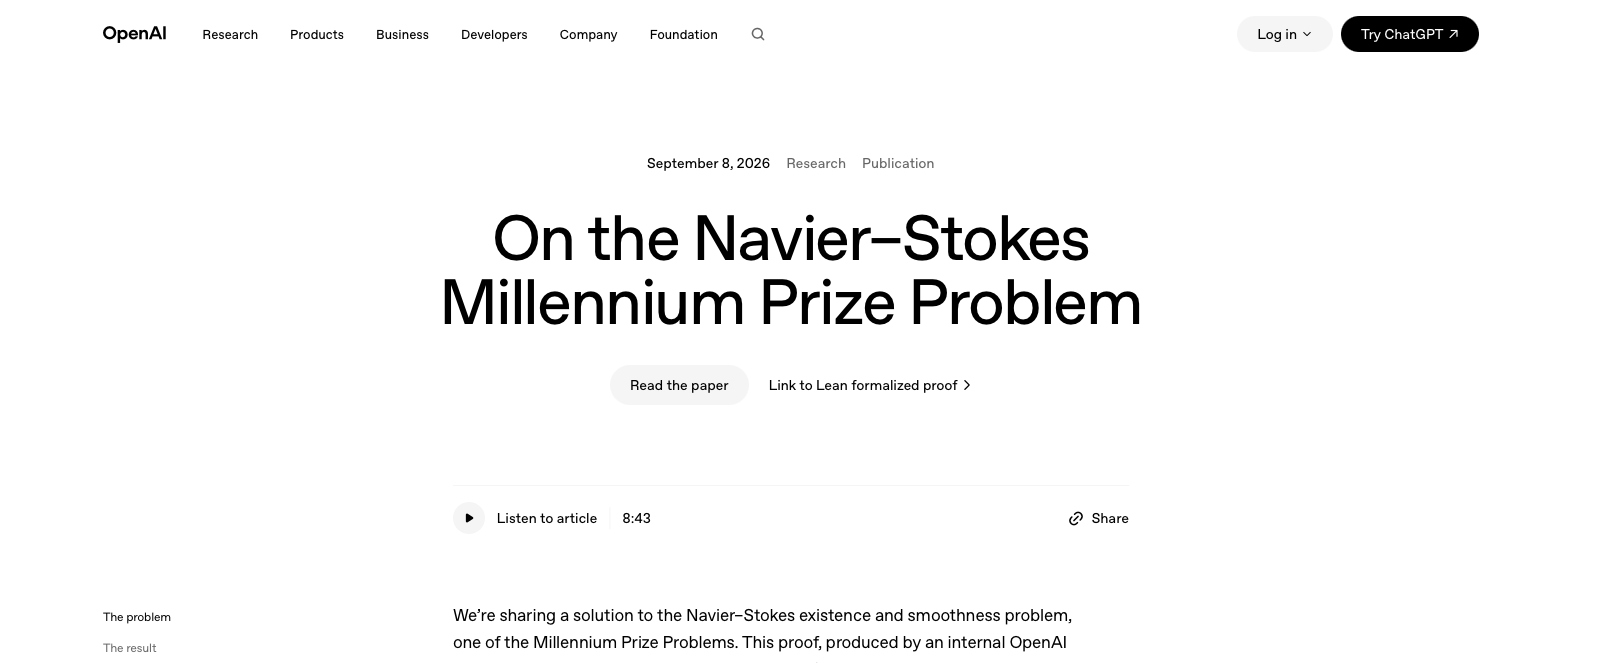
\includegraphics[width=0.95\textwidth]{NavierStokes.png}
  \end{center}
  \vfill
\end{frame}

%%%%%%%%%%%%%%%%%%%%%%%%%%%%%%%%%%%%%%%%%%%%%%%%%%%%%%%%%%%%%%%%%%%%%%%%%%%%%%%
%  3.  A RAPID OVERVIEW OF LEAN
%%%%%%%%%%%%%%%%%%%%%%%%%%%%%%%%%%%%%%%%%%%%%%%%%%%%%%%%%%%%%%%%%%%%%%%%%%%%%%%
\begin{frame}[fragile]{A rapid overview of Lean}
  \vfill
  \begin{columns}[c,onlytextwidth]

    \begin{column}{0.455\textwidth}
      \begin{plcard}[halign=center,top=5pt,bottom=5pt]%
                    {plnavy}{\hfill One way to check by computer\hfill}
        \plbody Definitions, theorems, proofs\\[2pt]
        {\color{plorange}$\downarrow$}\\[2pt]
        \textbf{consistency \& correctness, guaranteed}
      \end{plcard}

      \begin{plcard}[top=5pt,bottom=5pt,before skip=2pt]{plblue}{Built on type theory}
        \plbody
        Lean knows the \textbf{type} of everything, and checks
        that things have the type expected.\par
        \vspace{4pt}
        {\centering\plbody
          $\underbrace{p}_{\text{proof}}\,:\,\underbrace{P}_{\text{theorem}}
           \qquad
           \underbrace{7}_{\text{term}}\,:\,\underbrace{\mathbb{N}}_{\text{type}}$\par}
      \end{plcard}
    \end{column}

    \begin{column}{0.525\textwidth}
      \begin{plplain}[top=3pt,bottom=3pt]{plorange}
        {\pllabel\color{plember}A definition, a theorem, a proof}
        \vspace{3pt}
\begin{lstlisting}
def energy (m v : Real) : Real :=
  m * v ^ 2 / 2

theorem energy_nonneg
    (m v : Real) (hm : 0 <= m) :
    0 <= energy m v := by
  unfold energy
  positivity
\end{lstlisting}
      \end{plplain}
      \vspace{4pt}
      \begin{center}
        {\plmeta\color{white!85}\faIcon{globe}\;
          \href{https://live.lean-lang.org/\#codez=JYWwDg9gTgLgBAWQIYwBYBtgCMBQP0CmIIScwAdgMYTkDOwtMB5MA\%2BmgdEXABSkBccQCSEASl4AzOIMCohHEBJhHGljBkgLxwB6rAE84taFF15CxUgHcoNAObtUnKN0EAGOOoBMUrbv1RDcY0QkcNS\%2BBJRsHFwgvKRYwVLCyjFwANRwcWmUIgB6ACyuOHBFxUh5qellmXmFxUVpuQBUpQDMDRlwjS0NlDW19U1t2c3ljVhD3b3F\%2FUjdQyNts82TdXAAbE3ZboMeaeulW5Sb5etjB5vL5QCMW\%2FsLlFc3290PA1izHvxeNVAUVnjkNGo4AArjAkFhCHAACYESTMAhQKy6HjRABuCQASgQkOgklicZ4atEGnB0dk4B4APQUmo4SIOaLwxHaVgA8jkAhWXhozHY3G8VDRZxwAA86hAyhqLjFcCZSLgPM\%2B6W0NWB5HEEHQUNlHOZNUg9BgwFRwBg2iAA}%
            {\color{white!85}Open this example in the live editor}}
      \end{center}
    \end{column}

  \end{columns}
  \vfill
\end{frame}

%%%%%%%%%%%%%%%%%%%%%%%%%%%%%%%%%%%%%%%%%%%%%%%%%%%%%%%%%%%%%%%%%%%%%%%%%%%%%%%
%  4.  THE LEAN <-> AI FEEDBACK LOOP
%  AI generates, Lean checks; the verified output is what trains the next model.
%%%%%%%%%%%%%%%%%%%%%%%%%%%%%%%%%%%%%%%%%%%%%%%%%%%%%%%%%%%%%%%%%%%%%%%%%%%%%%%
\begin{frame}{Bringing AI in to the story}
  \vfill
  \begin{center}
  \begin{tikzpicture}[
      plbox/.style={rectangle, rounded corners=9pt, fill=white,
        line width=1.6pt, minimum width=4.4cm, minimum height=2.5cm, align=center,
        drop shadow={shadow xshift=1.4pt, shadow yshift=-1.8pt,
                     fill=black!70, opacity=0.35}},
      flow/.style={-{Stealth[length=4.2mm,width=3.2mm]}, line width=2.4pt},
      lab/.style={font=\bfseries\small, color=white, inner sep=3pt},
    ]

    \node[plbox, draw=plorange] (ai) at (-4.1,0)
      {{\color{plorange}\fontsize{31}{31}\selectfont\faIcon{robot}}\\[10pt]
       {\color{plnavy}\Large\bfseries AI}};

    \node[plbox, draw=plsky] (lean) at (4.1,0)
      {{\color{plblue}\fontsize{31}{31}\selectfont\faIcon{check-double}}\\[10pt]
       {\color{plnavy}\Large\bfseries Lean}};

    % AI -> Lean : the model writes candidate proofs
    \draw[flow, plorange] (ai.north) to[bend left=26]
      node[lab, above=1pt, midway] {generates} (lean.north);

    % Lean -> AI : the checker's verdict is training signal
    \draw[flow, plsky] (lean.south) to[bend left=26]
      node[lab, below=1pt, midway] {verifies} (ai.south);

  \end{tikzpicture}
  \end{center}
  \vfill
\end{frame}

%%%%%%%%%%%%%%%%%%%%%%%%%%%%%%%%%%%%%%%%%%%%%%%%%%%%%%%%%%%%%%%%%%%%%%%%%%%%%%%
%  4b.  THE CATCH -- CORRECTNESS IS NOT RELEVANCE
%  Lean checks the proof, never the statement: the definitions carry the meaning.
%%%%%%%%%%%%%%%%%%%%%%%%%%%%%%%%%%%%%%%%%%%%%%%%%%%%%%%%%%%%%%%%%%%%%%%%%%%%%%%
\begin{frame}[fragile]{There is a problem!}
  \vfill
  \begin{columns}[c,onlytextwidth]

    \begin{column}{0.415\textwidth}
      \begin{plcard}[top=9pt,bottom=9pt]{plember}{The catch}
        {\plbody Mathematical \textbf{correctness} and \textbf{consistency}
         do \emph{not} imply the mathematics is about the
         \textbf{right thing}.\par}
      \end{plcard}
    \end{column}

    \begin{column}{0.565\textwidth}
      \begin{plplain}[top=3pt,bottom=3pt]{plember}
        {\pllabel\color{plember}Fermat's Last Theorem, made trivial}
        \vspace{3pt}
\begin{lstlisting}
-- "the integers"
def MyInt : Type := Empty

def add (a b : MyInt) : MyInt :=
  Empty.elim a
def pow (a : MyInt) (n : Nat) : MyInt :=
  Empty.elim a

theorem fermat_last_theorem (a b c : MyInt)
    (n : Nat) (hn : 3 <= n) :
    Ne (add (pow a n) (pow b n)) (pow c n) :=
  Empty.elim a
\end{lstlisting}
      \end{plplain}
      \vspace{2pt}
      {\plmeta\color{white!85}\faIcon{check-double}\;
        Lean accepts it. Nothing here is about numbers.\par}
    \end{column}

  \end{columns}
  \vfill
\end{frame}

%%%%%%%%%%%%%%%%%%%%%%%%%%%%%%%%%%%%%%%%%%%%%%%%%%%%%%%%%%%%%%%%%%%%%%%%%%%%%%%
%  5.  WHAT MAKES THE LOOP WORK -- MATHLIB
%%%%%%%%%%%%%%%%%%%%%%%%%%%%%%%%%%%%%%%%%%%%%%%%%%%%%%%%%%%%%%%%%%%%%%%%%%%%%%%
\begin{frame}{What the loop is built on}
  \vfill
  \begin{center}
  \begin{tcolorbox}[enhanced, width=0.92\textwidth, arc=10pt, outer arc=10pt,
      colback=white, colframe=plrule, boxrule=1.2pt,
      left=18pt,right=18pt,top=14pt,bottom=14pt, drop fuzzy shadow={black!55}]
    \begin{minipage}[c]{0.10\textwidth}
      {\color{plmuted}\fontsize{30}{30}\selectfont\faIcon{github}}
    \end{minipage}\hfill
    \begin{minipage}[c]{0.70\textwidth}
      {\Large\bfseries\color{plnavy}leanprover-community\,/\,mathlib4}\\[4pt]
      {\plbody\color{plmuted}\raggedright A \emph{monolithic} library of
       mathematics formalized in Lean --- large enough to work at a high level.\par}
    \end{minipage}\hfill
    \begin{minipage}[c]{0.17\textwidth}
      \raggedleft\plchip{plgreen}{public}\\[3pt]\plchip{plnavy}{Lean 4}
    \end{minipage}

    \vspace{12pt}{\color{plrule}\rule{\linewidth}{0.8pt}}\vspace{7pt}

    % the row has to stay on one line, so it is set tight
    {\plmeta\color{plmuted}
      \tikz[baseline=-2pt]{\fill[plnavy] (0,0) circle (3.4pt);}\; Lean
      \hspace{0.5em}\faIcon{book}\;\textbf{100{,}000} definitions
      \hspace{0.5em}\faIcon{check}\;\textbf{200{,}000} theorems
      \hspace{0.5em}\faIcon{users}\;\textbf{500+} contributors
      \hspace{0.5em}\faIcon{clock}\;started 2017}
  \end{tcolorbox}
  \end{center}
  \vfill
\end{frame}

%%%%%%%%%%%%%%%%%%%%%%%%%%%%%%%%%%%%%%%%%%%%%%%%%%%%%%%%%%%%%%%%%%%%%%%%%%%%%%%
%  5b.  FERMAT'S LAST THEOREM FORMALIZATION SCREENSHOT
%%%%%%%%%%%%%%%%%%%%%%%%%%%%%%%%%%%%%%%%%%%%%%%%%%%%%%%%%%%%%%%%%%%%%%%%%%%%%%%
\begin{frame}{Formalizing Fermat's Last Theorem}
  \vfill
  \begin{center}
    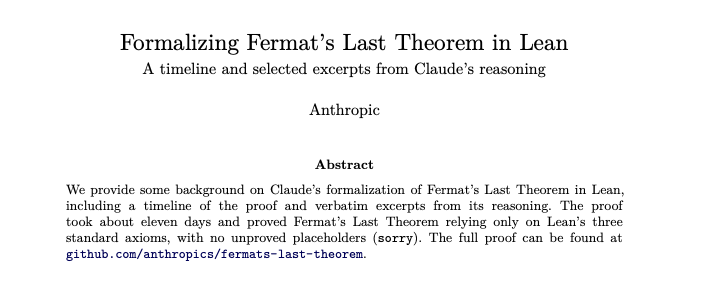
\includegraphics[width=0.95\textwidth]{FormalizationFermat.png}
  \end{center}
  \vfill
\end{frame}

%%%%%%%%%%%%%%%%%%%%%%%%%%%%%%%%%%%%%%%%%%%%%%%%%%%%%%%%%%%%%%%%%%%%%%%%%%%%%%%
%  6.  MY BROAD INTEREST -- PHYSLIB
%%%%%%%%%%%%%%%%%%%%%%%%%%%%%%%%%%%%%%%%%%%%%%%%%%%%%%%%%%%%%%%%%%%%%%%%%%%%%%%
\begin{frame}{My broad interest}
  \vfill
  \begin{center}
  \begin{tcolorbox}[enhanced, width=0.92\textwidth, arc=10pt, outer arc=10pt,
      colback=white, colframe=plrule, boxrule=1.2pt,
      left=18pt,right=18pt,top=14pt,bottom=14pt, drop fuzzy shadow={black!55}]
    \begin{minipage}[c]{0.10\textwidth}
      {\color{plmuted}\fontsize{30}{30}\selectfont\faIcon{github}}
    \end{minipage}\hfill
    \begin{minipage}[c]{0.70\textwidth}
      {\Large\bfseries\color{plnavy}leanprover-community\,/\,physlib}\\[4pt]
      {\plbody\color{plmuted}\raggedright A \emph{community-driven} project to
       digitalise results from physics into Lean.\par}
    \end{minipage}\hfill
    \begin{minipage}[c]{0.17\textwidth}
      \raggedleft\plchip{plgreen}{public}\\[3pt]\plchip{plnavy}{Lean 4}
    \end{minipage}

    \vspace{12pt}{\color{plrule}\rule{\linewidth}{0.8pt}}\vspace{7pt}

    {\plmeta\color{plmuted}
      \tikz[baseline=-2pt]{\fill[plnavy] (0,0) circle (3.4pt);}\; Lean
      \hspace{1.1em}\faIcon{star}\;\textbf{733} stars
      \hspace{1.1em}\faIcon{code-branch}\;\textbf{185} forks
      \hspace{1.1em}\faIcon{users}\;\textbf{100} contributors
      \hspace{1.1em}\faIcon{clock}\;started 2024}
  \end{tcolorbox}
  \end{center}
  \vfill
\end{frame}

%%%%%%%%%%%%%%%%%%%%%%%%%%%%%%%%%%%%%%%%%%%%%%%%%%%%%%%%%%%%%%%%%%%%%%%%%%%%%%%
%  6b.  WHAT PHYSLIB IS
%%%%%%%%%%%%%%%%%%%%%%%%%%%%%%%%%%%%%%%%%%%%%%%%%%%%%%%%%%%%%%%%%%%%%%%%%%%%%%%
\begin{frame}{What Physlib is}
  \vfill
  \setbeamercolor{normal text}{fg=white}
  \usebeamercolor*{normal text}
  \setbeamercolor{itemize item}{fg=plsky}
  \begin{center}
    \begin{minipage}{0.85\textwidth}
      \large
      \begin{itemize}
        \item A \textbf{monolithic library} for physics results from standard
          physics (not just axiomatisations).
        \item[] \vspace{4pt}
        \item Research-level results, with carefully standardized definitions
          and theorems --- a foundation for future formalization.
        \item[] \vspace{4pt}
        \item Community run (no bias to any academic or company), following
          open-source software workflows.
      \end{itemize}
    \end{minipage}
  \end{center}
  \vfill
  % restore, since setbeamercolor{normal text} + usebeamercolor* is global state
  \setbeamercolor{normal text}{fg=plink}
  \usebeamercolor*{normal text}
\end{frame}

%%%%%%%%%%%%%%%%%%%%%%%%%%%%%%%%%%%%%%%%%%%%%%%%%%%%%%%%%%%%%%%%%%%%%%%%%%%%%%%
%  6c.  STRUCTURE OF PHYSLIB
%%%%%%%%%%%%%%%%%%%%%%%%%%%%%%%%%%%%%%%%%%%%%%%%%%%%%%%%%%%%%%%%%%%%%%%%%%%%%%%
\begin{frame}{Structure of Physlib}
  \vfill
  \begin{center}
    {\pllabel\color{plsky!35!white} UPSTREAM}\quad
    {\color{white}\bfseries Mathlib}\\[2pt]
    {\color{plsky!40!white}\Large$\Downarrow$}\\[4pt]
    {\pllabel\color{plsky!35!white} THIS REPOSITORY}
  \end{center}

  \vspace{4pt}
  \begin{columns}[T,onlytextwidth]

    \begin{column}{0.315\textwidth}
      \begin{plcardh}{plorange}{\plchip{plorange}{CORE}}{2.95cm}
        \large\bfseries\color{plnavy}
        Physlib
        \par\vspace{4pt}
        {\plbody\normalfont\color{plink}Curated to a high standard for long-term reuse.}
      \end{plcardh}
    \end{column}

    \begin{column}{0.315\textwidth}
      \begin{plcardh}{plblue}{\plchip{plblue}{RAPID}}{2.95cm}
        \large\bfseries\color{plnavy}
        PhyslibAlpha
        \par\vspace{4pt}
        {\plbody\normalfont\color{plink}Lighter review, for large-scale AI-assisted contributions.}
      \end{plcardh}
    \end{column}

    \begin{column}{0.315\textwidth}
      \begin{plcardh}{plgreen}{\plchip{plgreen}{QI}}{2.95cm}
        \large\bfseries\color{plnavy}
        QuantumInfo
        \par\vspace{4pt}
        {\plbody\normalfont\color{plink}Quantum information theory, being brought closer to Physlib.}
      \end{plcardh}
    \end{column}

  \end{columns}
  \vspace{4pt}

  \begin{center}
    {\pllabel\color{plsky!35!white} ADJACENT}\quad
    {\color{plsky!40!white}\Large$\Rightarrow$}\quad
    {\color{white}\bfseries CSLib}
  \end{center}
  \vfill
\end{frame}

%%%%%%%%%%%%%%%%%%%%%%%%%%%%%%%%%%%%%%%%%%%%%%%%%%%%%%%%%%%%%%%%%%%%%%%%%%%%%%%
%  6d.  WHAT PHYSLIB CONTAINS
%%%%%%%%%%%%%%%%%%%%%%%%%%%%%%%%%%%%%%%%%%%%%%%%%%%%%%%%%%%%%%%%%%%%%%%%%%%%%%%
\begin{frame}{What Physlib contains}
  \vfill
  \begin{center}
    \begin{minipage}{0.92\textwidth}
      \centering
      \plchipbig{plblue}{ClassicalMechanics}\,
      \plchipbig{plblue}{Electromagnetism}\,
      \plchipbig{plblue}{Optics}\,
      \plchipbig{plblue}{Thermodynamics}\,
      \plchipbig{plblue}{StatisticalMechanics}\,
      \plchipbig{plblue}{CondensedMatter}\,
      \plchipbig{plblue}{FluidDynamics}

      \vspace{10pt}
      \plchipbig{plorange}{QuantumMechanics}\,
      \plchipbig{plorange}{QFT}\,
      \plchipbig{plorange}{LatticeQFT}\,
      \plchipbig{plorange}{Particles}\,
      \plchipbig{plorange}{ClassicalFieldTheory}\,
      \plchipbig{plorange}{StringTheory}

      \vspace{10pt}
      \plchipbig{plgreen}{Relativity}\,
      \plchipbig{plgreen}{Cosmology}\,
      \plchipbig{plgreen}{SpaceAndTime}\,
      \plchipbig{plmuted}{Mathematics}\,
      \plchipbig{plmuted}{Units}\,
      \plchipbig{plmuted}{Meta}
    \end{minipage}
  \end{center}
  \vfill
\end{frame}

%%%%%%%%%%%%%%%%%%%%%%%%%%%%%%%%%%%%%%%%%%%%%%%%%%%%%%%%%%%%%%%%%%%%%%%%%%%%%%%
%  6f.  INTERESTING RESULTS IN PHYSLIB
%%%%%%%%%%%%%%%%%%%%%%%%%%%%%%%%%%%%%%%%%%%%%%%%%%%%%%%%%%%%%%%%%%%%%%%%%%%%%%%
\begin{frame}[fragile]{Interesting results in Physlib}
  \vfill
  \setbeamercolor{normal text}{fg=white}
  \usebeamercolor*{normal text}
  \begin{columns}[T,onlytextwidth]

    \begin{column}{0.475\textwidth}
      \begin{itemize}
        \item[{\color{plgreen!45!white}\faIcon{check-circle}}] Classical harmonic oscillator
        \item[{\color{plgreen!45!white}\faIcon{check-circle}}] Quantum harmonic oscillator
        \item[{\color{plgreen!45!white}\faIcon{check-circle}}] Maxwell's equation
        \item[{\color{plgreen!45!white}\faIcon{check-circle}}] Lorentz group
        \item[{\color{plgreen!45!white}\faIcon{check-circle}}] Twin paradox
      \end{itemize}
    \end{column}

    \begin{column}{0.475\textwidth}
      \begin{itemize}
        \item[{\color{plgreen!45!white}\faIcon{check-circle}}] Tight binding chain
        \item[{\color{plgreen!45!white}\faIcon{check-circle}}] Anomaly cancellation
        \item[{\color{plgreen!45!white}\faIcon{check-circle}}] CKM matrix
        \item[{\color{plgreen!45!white}\faIcon{check-circle}}] Wick's theorem
        \item[{\color{plgreen!45!white}\faIcon{check-circle}}] String theoretic
      \end{itemize}
    \end{column}

  \end{columns}

  \vspace{10pt}
  \begin{center}
    {\plmeta\color{white!85}\faIcon{globe}\;
      \href{https://live.lean-lang.org/\#url=https\%3A\%2F\%2Fgithub.com\%2Fleanprover-community\%2Fphyslib\%2Fblob\%2Fmaster\%2FPhyslib\%2FClassicalMechanics\%2FHarmonicOscillator\%2FBasic.lean}%
        {\color{white!85}Example of classical harmonic oscillator}}
  \end{center}
  \vfill
  \setbeamercolor{normal text}{fg=plink}
  \usebeamercolor*{normal text}
\end{frame}

%%%%%%%%%%%%%%%%%%%%%%%%%%%%%%%%%%%%%%%%%%%%%%%%%%%%%%%%%%%%%%%%%%%%%%%%%%%%%%%
%  7.  ONGOING WORK -- FORMALIZING THE STANDARD MODEL
%%%%%%%%%%%%%%%%%%%%%%%%%%%%%%%%%%%%%%%%%%%%%%%%%%%%%%%%%%%%%%%%%%%%%%%%%%%%%%%
\begin{frame}{Ongoing work: Standard Model}
  \vfill
  \begin{plplain}[top=3pt,bottom=3pt]{plnavy}
    \vspace{1pt}
    \begin{align*}
      \mathcal{L}_{\text{SM}} \;=\;
        & -\tfrac{1}{4}\,G^{A}_{\mu\nu}G^{A\,\mu\nu}
          -\tfrac{1}{4}\,W^{I}_{\mu\nu}W^{I\,\mu\nu}
          -\tfrac{1}{4}\,B_{\mu\nu}B^{\mu\nu}
          \;+\;\sum_{\psi}\, i\,\bar{\psi}\,\gamma^{\mu}D_{\mu}\psi\\
        & +\,(D_{\mu}H)^{\dagger}(D^{\mu}H)
          \;+\;\mu^{2}\,H^{\dagger}H\;-\;\lambda\,(H^{\dagger}H)^{2}\\
        & -\,\Big(\bar{Q}_{L}\,Y_{u}\,\tilde{H}\,u_{R}
                 +\bar{Q}_{L}\,Y_{d}\,H\,d_{R}
                 +\bar{L}_{L}\,Y_{e}\,H\,e_{R}
                 +\text{h.c.}\Big)
    \end{align*}
    \vspace{-9pt}
  \end{plplain}

  \begin{plplain}[top=3pt,bottom=3pt,before skip=2pt]{plblue}
    {\scriptsize
    \vspace{-3pt}
    \begin{align*}
      D_{\mu} &= \partial_{\mu} - i g_{3} G^{A}_{\mu}T^{A}
                 - i g_{2} W^{I}_{\mu}t^{I} - i g_{1} Y B_{\mu}\,,
      \qquad
      B_{\mu\nu} = \partial_{\mu}B_{\nu}-\partial_{\nu}B_{\mu}\,,\\
      G^{A}_{\mu\nu} &= \partial_{\mu}G^{A}_{\nu}-\partial_{\nu}G^{A}_{\mu}
                 + g_{3} f^{ABC} G^{B}_{\mu}G^{C}_{\nu}\,,
      \qquad
      W^{I}_{\mu\nu} = \partial_{\mu}W^{I}_{\nu}-\partial_{\nu}W^{I}_{\mu}
                 + g_{2}\,\epsilon^{IJK} W^{J}_{\mu}W^{K}_{\nu}\,.
    \end{align*}
    \vspace{-12pt}}
    \begin{center}\scriptsize
      $G=SU(3)\times SU(2)\times U(1)$, acting on three generations of\\
      $Q_{L}(\mathbf{3},\mathbf{2})_{1/6}$,
      $u_{R}(\mathbf{3},\mathbf{1})_{2/3}$,
      $d_{R}(\mathbf{3},\mathbf{1})_{-1/3}$,
      $L_{L}(\mathbf{1},\mathbf{2})_{-1/2}$,
      $e_{R}(\mathbf{1},\mathbf{1})_{-1}$, and $H(\mathbf{1},\mathbf{2})_{1/2}$.
    \end{center}
  \end{plplain}
  \vfill
\end{frame}

%%%%%%%%%%%%%%%%%%%%%%%%%%%%%%%%%%%%%%%%%%%%%%%%%%%%%%%%%%%%%%%%%%%%%%%%%%%%%%%
%  APPENDIX -- OTHER WORK ON LEAN AT BATH
%%%%%%%%%%%%%%%%%%%%%%%%%%%%%%%%%%%%%%%%%%%%%%%%%%%%%%%%%%%%%%%%%%%%%%%%%%%%%%%
\begin{frame}{Other work on Lean at Bath}
  \vfill
  \begin{center}
  \begin{tcolorbox}[enhanced, width=0.85\textwidth, arc=10pt, outer arc=10pt,
      colback=white, colframe=plrule, boxrule=1.2pt,
      left=20pt,right=20pt,top=16pt,bottom=16pt, drop fuzzy shadow={black!55}]
    {\Large\bfseries\color{plnavy}Proof mining in Lean}\\[8pt]
    {\plbody\color{plink}\raggedright A library for partially automating the extraction of
     computational information from proofs, with a focus on convergence rates
     for optimization algorithms.\par}

    \vspace{12pt}{\color{plrule}\rule{\linewidth}{0.8pt}}\vspace{8pt}

    {\plmeta\color{plmuted}Thomas Powell \;\textbullet\; Ben Langton}
  \end{tcolorbox}
  \end{center}
  \vfill
\end{frame}

%%%%%%%%%%%%%%%%%%%%%%%%%%%%%%%%%%%%%%%%%%%%%%%%%%%%%%%%%%%%%%%%%%%%%%%%%%%%%%%
%  CLOSING
%%%%%%%%%%%%%%%%%%%%%%%%%%%%%%%%%%%%%%%%%%%%%%%%%%%%%%%%%%%%%%%%%%%%%%%%%%%%%%%
{
\setbeamertemplate{footline}{}
\begin{frame}[plain]
  \vfill
  \begin{center}
    {\color{white}\fontsize{36}{40}\selectfont\bfseries
      Thank you for watching\par}

    \vspace{0.50cm}

    
\begin{tikzpicture}
      \fill[plsky!75] (0,0) rectangle (2.5cm,2pt);
      \fill[plorange] (2.75cm,-3pt) circle (4.5pt);
      \fill[plsky!75] (3.2cm,0) rectangle (5.7cm,2pt);
    \end{tikzpicture}

    \vspace{0.50cm}

    {\color{plsky!25!white}\plbody Joseph Tooby-Smith\;\textbullet\;University of Bath\par}

    \vspace{0.40cm}

    {\color{white!85}\plmeta
      \href{https://github.com/leanprover-community/physlib}{%
        \color{white!85}\faIcon{github}\; \texttt{leanprover-community/physlib}}
      \qquad
      \href{https://josephtoobysmith.com/}{%
        \color{white!85}\faIcon{globe}\; \texttt{josephtoobysmith.com}}\par}
  \end{center}
  \vfill
\end{frame}
}

\end{document}
